\section{Entwurfsentscheidungen}
\label{sec:fachkonzept-entwurf}

\subsection{Einleitung}
Zur Erstellung eines Unternehmensplanspiels bedarf es - wie in jedem Prozess der Software-Erstellung - nach einer anfänglichen Analyse der benötigten Funktionalität, deren Ergebnisse in \ref{sec:fachkonzept-usecase} anhand eines Use Case Diagramms verkürzt dargestellt wurden, Entscheidungen zum grundlegenden Entwurf der Software. Diese Phase grenzt sich klar ab von den Entscheidungen zur Implementierung des Projekts, die in \ref{sec:fachkonzept-implementierung} erläutert werden, da sie sich auf einem höheren Abstraktionsniveau bewegt. Es geht hierbei nicht darum, die Lösung auf eine bestimmte Umsetzung hin zu optimieren, sondern die erkannten Anforderungen weitestgehend zu ermöglichen. Diese Entscheidungen sollen strukturiert werden mit Hilfe der Notation des UML Klassendiagramms.

Konkret bedeutet der höhere Abstraktionsgrad, dass Eigenheiten wie die System-Architektur (z.B. Client-Server-Architekter), die Persistierung von Daten oder die Benutzeroberfläche an dieser Stelle weder behandelt noch berücksichtigt werden sollen. Es wird vielmehr die Spielwelt, die eingefasst ist in einen Rahmen, der den Zugriff durch Spielleiter und Spieler von Außen ermöglicht, modelliert.

\begin{figure}[p]
\setlength\fboxrule{0pt}
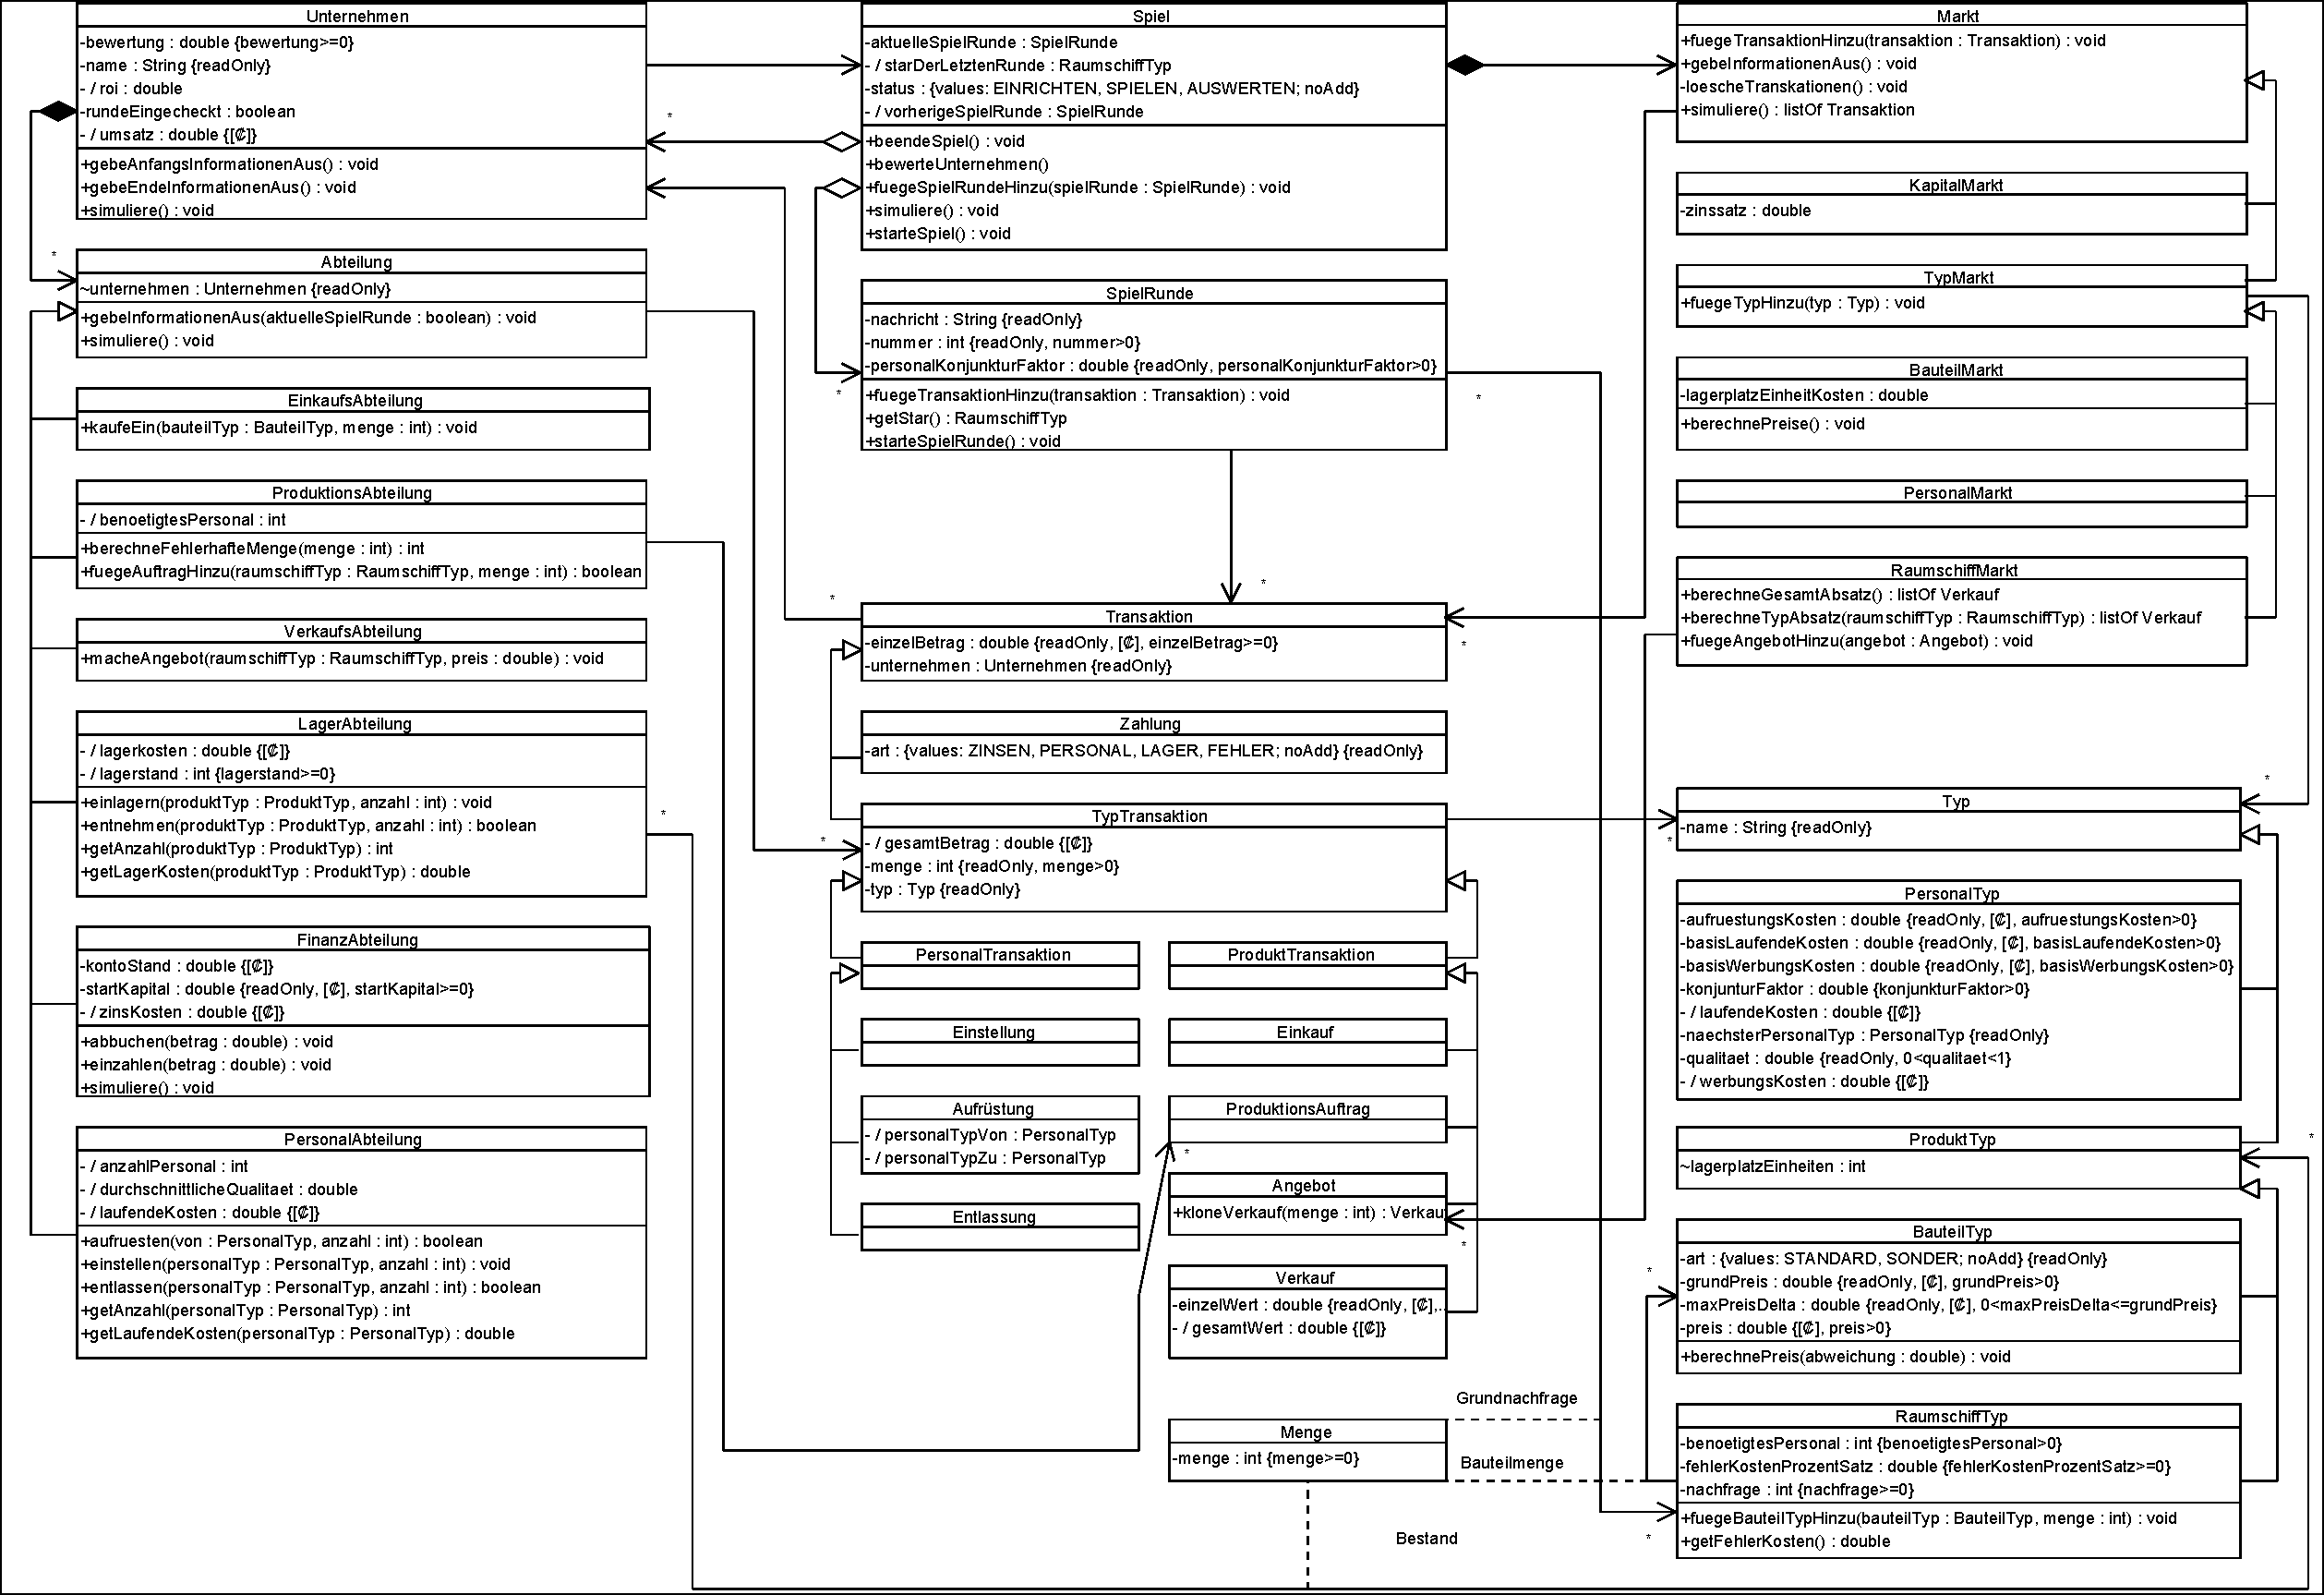
\includegraphics[angle=90, height=20cm]{30_Fachkonzept/20_Entwurf/gesamtmodell}
\caption{Klassendiagramm der Entwurfsphase}
\label{img:fachkonzept-entwurf-klassendiagramm}
\end{figure}

In \ref{img:fachkonzept-entwurf-klassendiagramm} ist das Klassendiagramm der Entwurfsphase dargestellt. Die Erstellung dieses Modell orientierte sich dabei zunächst an der erdachten Spielwelt. 

Spiel: zentrale Klasse
keine trivialen getter und setter

Im Folgenden sollen einige Bereiche aus diesem Modell getrennt voneinander betrachtet werden. Zunächst werden die sogenannten Typen, die Beschreibungen von konkreten Gegenständen der Spielwelt wie z.B. den Raumschifftypen darstellen, betrachtet. Daran schließt sich eine Erläuterung der Märkte an, gefolgt von einer Betrachtung der Klasse Unternehmen. Zuletzt werden die zur Erfassung der Vorgänge in der Spielwelt und deren Speicherung dienenden Transaktions-Klassen und die SpielRunde erörtert.

\subsection{Die Typen}
Der Begriff \textit{Typen} bezeichnet, wie oben bereits erwähnt, eine Beschreibung von einer Gruppe von Gegenständen der Spielwelt. Es wurde bewusst auf eine Modellierung jedes einzelnen Objekts in der Spielwelt verzichtet, um die Anzahl der benötigten Objekte nicht Überhand nehmen zu lassen. Obgleich diese Entscheidung vielleicht wie ein Vorgriff auf den Abstraktionsgrad der Implementierung wirkt, wurde hierdurch versucht, die Schere zwischen dem Modell der Entwurfs- und dem der Implementierungsphase möglichst gering zu halten, vor allem da sich die gewählte Möglichkeit nicht negativ auf die Funktionalität auswirkt. Die Gemeinsamkeit, die allen Typen innewohnt, ist der Name, der daher in einer Oberklasse definiert wurde.

Erkannt und umgesetzt wurde dabei die folgenden Typen, die ihrerseits von der Klassen \textit{Typ} erben:
\begin{seList}
\item \textbf{PersonalTyp:} Die für das Spiel notwendigen Personaltypen zeichnen sich einerseits durch ihren Qualitätsgrad, der die entstehenden Fehlerkosten beeinflusst, und andererseits durch die mit ihnen verbundenen Kosten aus. Hierzu gehören die Werbungskosten, die laufenden Kosten sowie die Schulungskosten, wobei die ersten zwei abhängig von der Konjunktur auf dem Personalmarkt variieren können.
\item \textbf{BauteilTyp:} In der Spielwelt des Planspiels können Bauteiltypen entweder die Rolle von Standard- oder Sonderbauteilen annehmen, wobei erstere für jeden Raumschifftyp benötigt werden. Da dies in der Berechnung der neuen Bauteilpreise berücksichtigt werden muss, wird diese Eigenschaft abgespeichert.
\item \textbf{RaumschiffTyp:}
\end{seList}

Synergie ProduktTyp

\subsection{Die Märkte}
Aus der Definition des Spielszenarios lassen sich folgende Märkte ableiten:
\begin{seList}
\item \textbf{Raumschiffmarkt:} Dieser Markt ist vermutlich derjenige, der sich bei der Betrachtung von Raumschiffproduktions-Unternehmen in den Vordergrund drängt. Es handelt sich für die Spieler um den Absatzmarkt, an dem sie Verkaufsangebote machen können, die sich durch eine Menge und einen Preis auszeichnen. Alle Angebote, die im Laufe Runde gemacht werden, müssen zwischengespeichert und zum Schluss der Runde ausgewertet werden, um die Absatzwerte berechnen zu können. Zusätzlich verwaltet der Raumschiffmarkt alle Raumschifftypen der Spielwelt.

Referenz auf die Felder / Methoden.
\item \textbf{Bauteilmarkt:} Ähnlich
\end{seList}

Synergien!?

\subsection{Das Unternehmen}

\subsection{Spielrunde und Transaktionen}